\documentclass{article}
\usepackage{paquetes}

\begin{document}

\maketitle

\begin{abstract}

    \noindent Multiple individuals in cities and countries in the developing world suffer from constraints derive from access to equal opportunities. This constraints could affect labour market outcomes in different mechanisms. This paper focuses on two instruments on the labour market: no access to available information on vacants and distance limitations given nearby settlements to the city. Using experimental data on two different interventions (employment workshop and transport subsidies) in the city of Addis Ababa, Ethiopia, the authors compare labour market outcomes within treatment branches and across treatment groups. Results show that the employment intervention has more long lasting effects on working status probability, incomes and call backs for interviews than the subsidies intervention. However, both interventions improve labour market outcomes in the treatment group compared to the control group. Furthermore, effects on the transport subsidies rapidly disappear when treatment is terminated, but workshop effect could still be captured four years after the treatment finishes. My objective in this project will be to reproduce all results in \cite{abebe2021anonymity} and it´s Supplementary Online Annex. In doing so I will be assessing the quality of the reproduction package and will be commenting on improvements that the code and the organization of the project could have taken in order to make it more straightforwardly used. Lastly, some changes are produced in some of the paper tables and figures. The project is organized as follows. Section \ref{DF Previuos work} describes previous work done in assessing the reproduction package such as describing the paper, assigning score tot eh reproduction package and commenting on changes or improvement on the code. Section \ref{What´s next?} documents principal results such as tables and figures in the main and online annex. 
    
    
\end{abstract}

\newpage 

\noindent The repository which holds original and proposed replication files could be found in the following \href{https://github.com/jorgeluis8ar/Revised-reproduction-package-for-Abebe-et-al-2021}{link}. In order to get the results outlined in this file you should use all Do-Files in the \href{https://github.com/jorgeluis8ar/Revised-reproduction-package-for-Abebe-et-al-2021/tree/main/Proposed\%20Replication\%20File}{Proposed Replication File} folder and set the directory to where the folder will be stored.

\section{Previous work} \label{DF Previuos work}

    \subsection{Deliverable 1 - Brief explanation} \label{DF Deliverable 1}
    
    The paper focuses on two main research questions. First, what is the effect of interventions designed to reduce labour market frictions? Second, do signaling interventions have higher impact than transport subsidies in labour market outcomes? In order to answer the research questions, the authors use experimental data on two different interventions (employment workshop and transport subsidies) in the city of Addis Ababa, Ethiopia. In addition, using a theoretical labour market model framework, the empirical strategy used provides suggestive evidence on the compliance of four predictions. These predictions are:

    \begin{enumerate}
    
        \item \underline{\textbf{\textit{Effect on formal employment}}}: Both interventions will decrease formal unemployment rates. However, once treatment is over the effect will gradually disappear.
        
        \item \underline{\textbf{\textit{Search intensity and efficiency}}}: The transport intervention will increase the number of seen vacants. On the other hand, the employment workshop increases the probability of landing a job after finding a vacant.
        
        \item \underline{\textbf{\textit{Quality of the employee-employer match}}}: The employment workshop  generates a consistent increase in quality match; transport subsidies do not.
        
        \item \underline{\textbf{\textit{heterogeneous effects}}}: Individuals with worse observables will have higher impacts on either treatment branch.
        
    \end{enumerate}    
    
    \noindent The empirical strategy used in the paper is easy: simple means comparison using OLS. Two specifications are presented. First, the following static equation help to retrieve the effects of the treatment branches on labour market outcomes.
  
    \begin{equation}
        y_{ic} = \beta_0 + \sum_{f}\left[\beta_f\times \text{treat}_{fic} + \gamma_f\times\text{spillover}_{fic}\right] +\alpha \times y_{ic,\text{pre}} + \delta\times \mathbf{x}_{ic0} + \mu_{ic} \label{eq: DF main}
    \end{equation}  
    
    \noindent Second, a dynamic equation helps to obtain the dynamic effects in short, medium and long tern horizons. 
    
    \begin{equation}
        y_{itc} = \sum_{f} \sum_{w=S_f}^{E_f}\left[\beta_{fw}\times\text{treat}_{fic}\times d_{wit}+\gamma_{fw}\times\text{spillover}_{fic}\times d_{wit}\right] + \alpha_t\times y_{itc,\text{pre}} + \delta\times\mathbf{x}_{ic0} + \eta_t + \mu_{itc} \label{eq:DF second}
    \end{equation}
    
    \noindent Where $y_{ic}$ is a labour market outcome for individual $i$ in cluster $c$. $f$ stands for treatment branches, $t$ for a time subscript and$w$ stands for weeks. $\text{treat}_{fic}$ is a indicator variable equal to one if individual $i$ of cluster $c$ was randomly assigned to treatment branch $f$, zero otherwise. Main results and concussion come from specification \ref{eq: DF main}. 
    
    \subsection{Deliverable 2 - Reproduction score} \label{DF Deliverable 2}
    
    The reproduction package has the following structure:

    \begin{itemize}
        \item Data
        \item Do Files
        \item Figures
        \item Tables
        \item Utilities
    \end{itemize}
    
    \noindent The reproduction package in all is organized in a proficient way. All tables and figures are well documented in the Do Files and names are designed accordingly to results in the paper. But, there is still room for improvement. First, the main problem comes from understanding all the programs and ado files needed to run the scripts. Given that some packages are hard to find for \texttt{STATA} implementations, when trying to run all Do Files, there are several errors. This leads to inefficiency in terms of time used for understanding the structure. One possible solution is to create a Do file with all the installation commands for all the programs and functions needed for the analysis. Second, some Do Files called upon each other several times. This dynamic leads to uncertainty which data sets are used (could no make all the data connections allowed), so final conclusions on what data produces which figure or table does no have 100 \% accuracy. One solution would be to create a Do File with all the needed functions, program needed a just call a single data set and Do File to be sure what produces what. This caveats seem small, compared to the scale of the research project, but since there is room for improvement, I can not give a perfect score. Another small issue is that results in the corresponding tables are not a 100 percent identical. Described my comments, I can now score the reproduction package for display items. Given the size of the display items is remarkable, and that figures and tables are basically produced by the same commands, I decide to give an overall score to the reproduction package and not item by item. The score I give for the reproduction package of \cite{abebe2021anonymity} is 9 (L9). The reasons are explained above and given the space for improvement, a perfect score is not on the table.

    
    \subsection{Deliverable 3 - Code improvements} \label{DF Deliverable 3}


    For this third deliverable I edited and commented the existing code. To access the commit click on the commit's name. All commits are summarized in the following lists:

    \begin{itemize}
    
        \item \href{https://github.com/jorgeluis8ar/Revised-reproduction-package-for-Abebe-et-al-2021/commit/db2f73317a593a30509195413c5c7fff3020f6f0}{Initial commit} (tag: db22f733): This is the initiation commit for the repo.
        
        \item \href{https://github.com/jorgeluis8ar/Revised-reproduction-package-for-Abebe-et-al-2021/blob/main/Proposed\%20Replication\%20File/do/main_endline_results.do}{main\_end\_line\_results.do}: This Do File calls programs from the \href{https://github.com/jorgeluis8ar/Revised-reproduction-package-for-Abebe-et-al-2021/tree/main/Proposed\%20Replication\%20File/utilities}{Utilities} folder to make figures and tables using the end line results. This is the main script. The proposed changes or comments to the file are the following:
        
            \begin{enumerate}[label=\roman*]
            
                \item \href{https://github.com/jorgeluis8ar/Revised-reproduction-package-for-Abebe-et-al-2021/commit/d5c11dcb7b29ba319e42c9d09c46756ca05923f4}{Changed lines of code for loops to create tables 5 and 6 and some organization} (tag: d5c11dc): This commit gives better organization to the Do File and creates a loop to create Tables 5 and 6. This tables were scattered over the Do File.
                
                \item \href{https://github.com/jorgeluis8ar/Revised-reproduction-package-for-Abebe-et-al-2021/commit/a572971f09dbdd7fecb0b114e18fbccaf0c7d5d7}{Commenting on Table A.9 - Regressions} (tag: a572971): This commit makes comments on all the code preceding the output of table A.9. The table presents evidence on the predictors of take-up of treatment. In detail, the Do File runs two regressions each for each branch of treatment. In other words, the regressions try to provide evidence of self selection of individuals into the treatment. In the comment, the regressions are fully explained.
                
                \item \href{https://github.com/jorgeluis8ar/Revised-reproduction-package-for-Abebe-et-al-2021/commit/8d01994ec7aae7555512a7db8c3aa07e08492e41}{Creation of table A.12 and quantile regression comments} (tag: 8d01994):This commit produces table a12 that was not within the original replication files. I created matrices and stored results from quantile regression in a matrix. Consequently, the matrices are merged together and the final table a12 is produced. There are also some comments on quantile regression.
                
                \item \href{https://github.com/jorgeluis8ar/Revised-reproduction-package-for-Abebe-et-al-2021/commit/de6c56101850e92d42a961a6d413bd8c84734601}{Creation of table A.13 and quantile regression comments} (tag: de6c561):This commit produces table a13 that was not within the original replication files. I created matrices and stored results from quantile regression in a matrix. Consequently, the matrices are merged together and the final table a13 is produced. There are also some comments on quantile regression.
                
                \item \href{https://github.com/jorgeluis8ar/Revised-reproduction-package-for-Abebe-et-al-2021/commit/b872bb2c72623db8017084a556cd8e0cae2cb34a}{Renaming and reordering figure 3 to figure 1} (tag: b872bb2): This commit fixes a bug in the replication files. In detail, figure 1 in the original files was named as figured 3.  I fixed the bug and comment on what the code section is doing.
                
            \end{enumerate}
            
        \item \href{https://github.com/jorgeluis8ar/Revised-reproduction-package-for-Abebe-et-al-2021/blob/main/Proposed\%20Replication\%20File/do/bounds.do}{bounds.do}: This Do File processes data and creates tables a.8, a.27 - a.33. The proposed changes or comments to the file are the following:
        
            
            \begin{enumerate}[label=\roman*,resume]
            
                \item \href{https://github.com/jorgeluis8ar/Revised-reproduction-package-for-Abebe-et-al-2021/commit/19ff77e1dff8fdcff0cef8b42f2240cebde55e69}{Attrition analysis table A.8} (tag: 19ff77e): This commit comments and interprets regressions of table a.8. This table shows results on the predictors of attrition in the sample. The model is a Linear Probability Model for each of the follow up periods; end line 1 (2 years after the intervention) and end line 2 (6 years after the intervention).
                
                \item \href{https://github.com/jorgeluis8ar/Revised-reproduction-package-for-Abebe-et-al-2021/commit/623b13491d86c3642d111acb86e442946c3f2350}{Lee Bounds and table a.33} (tag: 632b134): This commit comments on the estimations presented in table a.33. In detail, the table presents estimates of lee bounds for the treatment effects of the two treatment branches in terms of formal work (written employment agreement) and permanent work.
                
            \end{enumerate}
            
        \item \href{https://github.com/jorgeluis8ar/Revised-reproduction-package-for-Abebe-et-al-2021/blob/main/Proposed\%20Replication\%20File/do/spillovers.do}{spillovers.do}: This Do File processes data and creates tables a.35 and a.36. The proposed changes or comments to the file are the following:
        
            \begin{enumerate}[label=\roman*,resume]
            
                \item \href{https://github.com/jorgeluis8ar/Revised-reproduction-package-for-Abebe-et-al-2021/commit/c1222935e2bf0b50c2eb634b05204e26f6625980}{Frisch-Waugh-Lovell and spillover effects} (tag: c122293): This commit comments on the estimates presented in tables a35 and a36. This tables calculate the spillover effect of the transport treatment on the treated and the untreated. In terms of the regression, the authors use the Frisch-Waugh-Lovell theorem to partial out covariates and keep the coefficients of interest.
                
            \end{enumerate}
        
        \item \href{https://github.com/jorgeluis8ar/Revised-reproduction-package-for-Abebe-et-al-2021/blob/main/Proposed\%20Replication\%20File/do/mediation_analysis.do}{mediation_analysis.do}: This Do File processes data and creates tables a.35 and a.36. The proposed changes or comments to the file are the following:
    
            \begin{enumerate}[label=\roman*,resume]
            
                \item \href{https://github.com/jorgeluis8ar/Revised-reproduction-package-for-Abebe-et-al-2021/commit/510393cf5a80245095b881ccb230c5c3905f2f05}{Frisch-Waugh-Lovell and determinants of 2018 wage earnings} (tag: 510393c): This commit comments on the estimates presented in tables a24. This tables calculate the determinants of 2018 wage earnings. In terms of the regression, the authors use the Frisch-Waugh-Lovell theorem to partial out covariates and keep the coefficients of interest and use different specification to see how estimators progress as new variables are introduced.
                
                \item \href{https://github.com/jorgeluis8ar/Revised-reproduction-package-for-Abebe-et-al-2021/commit/58766b37ea6cfac637cf7145a142e087f2c0e8e7}{Figure 4 - Regression analysis and code description} (tag: 58766b3): This commit comments on the estimates presented in figure 4. This figure analyses a mediation analysis of the determinants of wage earnings in end line number 2 (6 years after the intervention). The comments resumes the strategy (code wise) to get the estimates and the linear combinations to determine the point estimates and their confidence intervals. Furthermore, I also realise a brief analysis of the regression that produces such results.
                
            \end{enumerate}   
            
        \item \href{https://github.com/jorgeluis8ar/Revised-reproduction-package-for-Abebe-et-al-2021/blob/main/Proposed\%20Replication\%20File/utilities/_itt_bothendlines.do}{\_itt\_bothendlines.do}: This Do File creates the program that produces Table 2 of the paper. The proposed changes or comments to the file are the following:
        
            \begin{enumerate}[label=\roman*,resume]
            
                \item \href{https://github.com/jorgeluis8ar/Revised-reproduction-package-for-Abebe-et-al-2021/commit/00e24c30c18470bd7ba3a671a93adb63077e9afe}{Stata conditional trick and regression discussion and some organizing} (tag: 00e24c3): This commit introduces a cool stata programming trick to get two cases to run in the same loop. Especially, if there exist a variable in the data set, the program should run a regression, but if a variable is not in the data set, then the program should run a different specification.  I also describe the regression used to get results. This description has sub-sampling, weights, cluster standard errors and the use of locals to get the right specification.
                
                \item \href{https://github.com/jorgeluis8ar/Revised-reproduction-package-for-Abebe-et-al-2021/commit/653cfd44a4b794d232ddeaa8e165691c94b2622e}{Final comments on the matrix filling and the construction of linear hypotheses testing per period} (tag: 653cfd4): This commit gives the final comments of the matrices and gives comments on the construction of linear hypotheses testing for every of the end line periods.
                
                \item \href{https://github.com/jorgeluis8ar/Revised-reproduction-package-for-Abebe-et-al-2021/commit/871feb1a4f6ccdebbcbd5250ddb309804220a147}{Q-values and final comments on the program} (tag: 871feb1): This commit gives comments on what going on in the definition of the Q-values in a two step methodology. Finally, all the process of the program is outlined for further reproduction.
                
            \end{enumerate}
            
        \item \href{https://github.com/jorgeluis8ar/Revised-reproduction-package-for-Abebe-et-al-2021/blob/main/Proposed\%20Replication\%20File/utilities/_itt_oneendline.do}{\_itt\_oneendline.do}: This Do file creates the program that produces Table 3 of the paper. The proposed changes or comments to the file are the following:
        
            \begin{enumerate}[label=\roman*,resume]
            
                \item \href{https://github.com/jorgeluis8ar/Revised-reproduction-package-for-Abebe-et-al-2021/commit/ce7b2d1546f0be8c1006b62b1fcb8fa08944bc8f}{Cool programming trick and Table 3 regression description} (tag: ce7b2d1): This commit comments on a cool trick in stata in order to account for different cases extending from a command. Example: types of variables. Whether a variable is string or numeric, the program does two different things. In the code the authors use to run regressions whether the variables exists or not.
                
                \item \href{https://github.com/jorgeluis8ar/Revised-reproduction-package-for-Abebe-et-al-2021/commit/deddd0e0e7c3b0dc6bd1a2ce24abf29283bc6d8e}{Final description of the Do File and scratching off unused lines} (tag: deddd0e): This commit comprises the final complete description of the function, scratching off unused lines in the code and changes in the Do File. 
                
            \end{enumerate}
    
        \item \href{https://github.com/jorgeluis8ar/Revised-reproduction-package-for-Abebe-et-al-2021/blob/main/Proposed\%20Replication\%20File/utilities/_itt_het.do}{\_itt\_het.do}: This Do file creates the program that produces Tables 4,5,6 and A.26 of the paper and online annex. The proposed changes or comments to the file are the following:
        
            \begin{enumerate}[label=\roman*,resume]
            
                \item \href{https://github.com/jorgeluis8ar/Revised-reproduction-package-for-Abebe-et-al-2021/commit/d6b2a2e8158fab04975ec35186ddacc6c33c7357}{Cool Stata programing trick, regression description and modifying the output of the program} (tag: d6b2a2e): This commit comments on a cool trick used in Stata. In detail, the authors use it to account for the non existence of a baseline variable. If it does exists, the program runs a different specification that if it does no exist. I also describe the regression specification and explain what is been used in each option. Finally I propose a small change of the program so it does not print every single step of the loop.
                
                \item \href{https://github.com/jorgeluis8ar/Revised-reproduction-package-for-Abebe-et-al-2021/commit/022d67398d62c3d46974c861532ff0fa189ca29a}{Final comments on the matrices filling, modifying the program output} (tag: 022d673): This commit gives the finals comments on the matrices filing and modifies the program so not every step of the loops gets printed.
                
                \item \href{https://github.com/jorgeluis8ar/Revised-reproduction-package-for-Abebe-et-al-2021/commit/39a899a7236ea5c4388241921f426cc96647fd73}{Q-values and finals comments in all the program} (tag: 39a899a): This commit gives comments on what going on in the definition of the Q-values in a two step methodology. Finally, all the process of the program is outlined for further reproduction.
                
            \end{enumerate}
        
        \item \href{https://github.com/jorgeluis8ar/Revised-reproduction-package-for-Abebe-et-al-2021/blob/main/Proposed\%20Replication\%20File/utilities/_itt_onetreat.do}{\_itt\_onetreat.do}: This Do File create the program that produces tables A.29-A.32 of the online annex. The proposed changes or comments to the file are the following:
    
            \begin{enumerate}[label=\roman*,resume]
            
                \item \href{https://github.com/jorgeluis8ar/Revised-reproduction-package-for-Abebe-et-al-2021/commit/9611d540c46597e748a5878ead0ce6f49d80889d}{Cool stata coding trick and regression analysis explanation} (tag: 9611d54): This commit comments on a Stata coding trick, but mainly it describes the regression analysis that is done. As a difference on previous estimations, this regressions takes a dummy variable as the intention to treatment if the individual was ever assigned to any treatment group.
                
                \item \href{https://github.com/jorgeluis8ar/Revised-reproduction-package-for-Abebe-et-al-2021/commit/60b06721ee8e688e123f523b3c04092f99dadd1b}{Final comments on the matrices filling, modifying the program output} (tag: 60b0672): This commit gives the finals comments on the matrices filing and modifies the program so not every step of the loops gets printed. Also I delete some parts of the code that did nothing and do not affect the end result.
                
                
            \end{enumerate}
    \end{itemize}


\section{What´s next?} \label{What´s next?}
\subsection{Tables}
In this final deliverable I will show some tables and figures with some comments and some changes that might feel the paper more suitable for reading. The first change I made is to change the statistical significance symbols used. The main reason is to show that I have a complete understanding of the reproduction package. The new values are as follows:

\medskip

\begin{table}[h!]
    \centering
    \caption{Original and proposed statistical symbols}
    \begin{tabular}{|c|c|c|}
    \hline
      \textbf{Confidence level} & \textbf{Original symbol} & \textbf{Proposed symbol}\\
    \hline
        1\%   & *** & • \\
    \hline
         5 \% &  ** & † \\
    \hline
        10 \% &  *  & § \\    
    \hline
    \end{tabular}
    \label{tab:my_label}
\end{table}


%% Table 2 of Abebe et al (2021) ----------------------------------------------

\import{Final Project/Deliverable Final/Tables/Original/}{table2}\label{tab:FD table 2 o}
\import{Final Project/Deliverable Final/Tables/Proposed/}{table2}\label{tab:FD table 2 p}

\noindent Tables \ref{tab:FD table 2 o} and \ref{tab:FD table 2 p} show the comparisons of the original papers tables format and the format I proposed for the replication file. Beyond aesthetics changes, Table \ref{tab:FD table 2 o} shows the effect of the treatment branches on labour market outcomes. In detail, the table presents Intention to Treatment (ITT) effects in both experiment end lines. The table is organized to show comparisons of treatment effects within end lines. This format helps to answer one of the research questions. When looking at column 4, one of the first results is that there are not statistical differences in almost all labour market outcomes, but in permanent work status. Thus, both interventions increased the probability of work, the total hours of work, labour incomes, and formal work probability. Furthermore, when looking at column 8, the main results of the paper appear. Employment workshop interventions effects tend to stay on time, while transport subsides are temporary and disappear rapidly. Only two labour market outcomes do not show statistical differences across treatment branches in the second end line. Individuals who were assigned to the employment workshop intervention have higher work probability, work more hours, earn higher labour incomes and report to be more satisfied with current work.

\medskip

%% Table 3 of Abebe et al (2021) ----------------------------------------------

\import{Final Project/Deliverable Final/Tables/Original/}{table3}\label{tab:FD table 3 o}

\noindent Now, when looking at match quality indicator of employer and employee match quality, I turn into Tables \ref{tab:FD table 3 o} and \ref{tab:FD table 3 p}. Column 5 shows the differences of treatment effects on match quality. Results show that tenure time, skills used at jobs and promotions status do not differ across treatment branches. However, when we talk about wages and the longest tenure, the employment workshop has higher effects than the transport subsidies intervention. In detail, when looking at the differences in wages, the workshop intervention has a higher effect over 5 to 6 times over the transport subsidy intervention. 

\import{Final Project/Deliverable Final/Tables/Proposed/}{table3}\label{tab:FD table 3 p}

%% Table 4 of Abebe et al (2021) ----------------------------------------------

\noindent Tables \ref{tab:FD table 4 o} and \ref{tab:FD table 4 p} shows comparisons of treatment effects across several different baseline covariates in the second end line. This exercise is supposed to suggest experimental heterogeneous evidence of prevalent characteristics for individuals. This treatment effects are presented for both treatment branches. Finally, columns 7 and 8 show p value for t-test of estimates for equality of effects in columns 2, 3, 5, and 6. Thus, the p-value show statistically differences in treatment effect for people of different baseline characteristics. Variables coded as 0 refers to the group that, in general, might be expected to face greater labour market disadvantage. The main result is that treatment effect, no matter treatment branch, are statistically higher for unfavorable individuals. For example, job seekers without tertiary education experience an effect of about 60\% of the control mean.

\import{Final Project/Deliverable Final/Tables/Original/}{table4}\label{tab:FD table 4 o}

\noindent Now, when looking at people who have ever been involved in the labour market, treated individuals experience a 22\% effect compared to the control mean. When comparing into intervention types, the workshop and transport subsidy have equal within treatment effect but in tertiary education and ever had a permanent job. 

\import{Final Project/Deliverable Final/Tables/Proposed/}{table4}\label{tab:FD table 4 p}

\newpage
%% Table 5 of Abebe et al (2021) ----------------------------------------------

\noindent Tables \ref{tab:FD table 5 o} and \ref{tab:FD table 5 p} follows the same structure of the previous tables but focuses on short term outcomes (first end line). In detail, the tables show results on permanent job status. The authors find that the effects on permanent work are significantly larger for individuals who have no tertiary education and larger in magnitude for individuals with no job experience in permanent employment.

\import{Final Project/Deliverable Final/Tables/Original/}{table5}\label{tab:FD table 5 o}
\import{Final Project/Deliverable Final/Tables/Proposed/}{table5}\label{tab:FD table 5 p}

\noindent For further comparison on tables  of the original and proposed changes see section \ref{apendix tables} of the appendix.

\newpage

\subsection{Figures}

Now, in terms of figures, I decided to change the background and delete all vertical and horizontal lines. The criteria to make this changes is purely aesthetics. One little caveat comes when proposing my graphs. All text such as titles, subtitles, axis titles, axis tick and legend text is shift to one side and does not fit the graph regions. This problem is a special feature of my computer. 

\begin{figure}[h!]
\censubtering
  \subfloat[Original \label{fig: figure 1 o}]{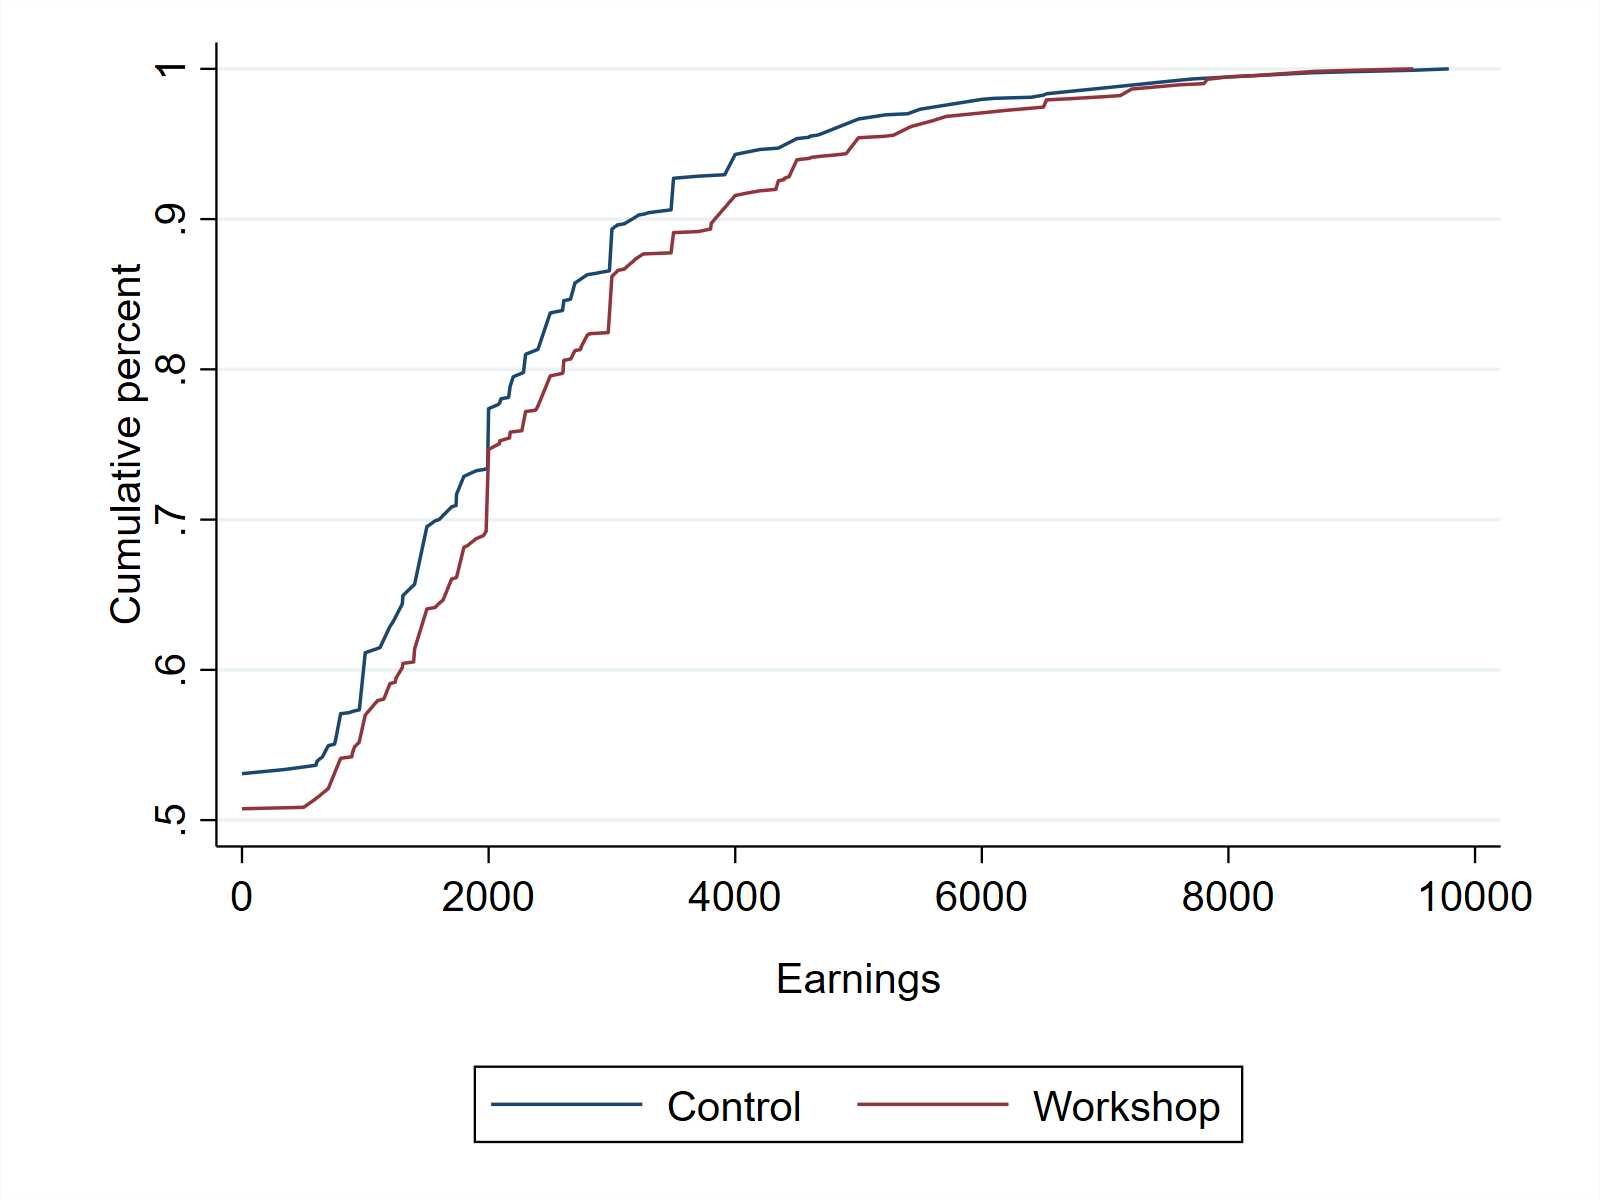
\includegraphics[width=7.5cm,height=5.0cm]{Final Project/Deliverable Final/Figures/Original/figure3.png}}\qquad
  \subfloat[Proposed \label{fig: figure 1 p}]{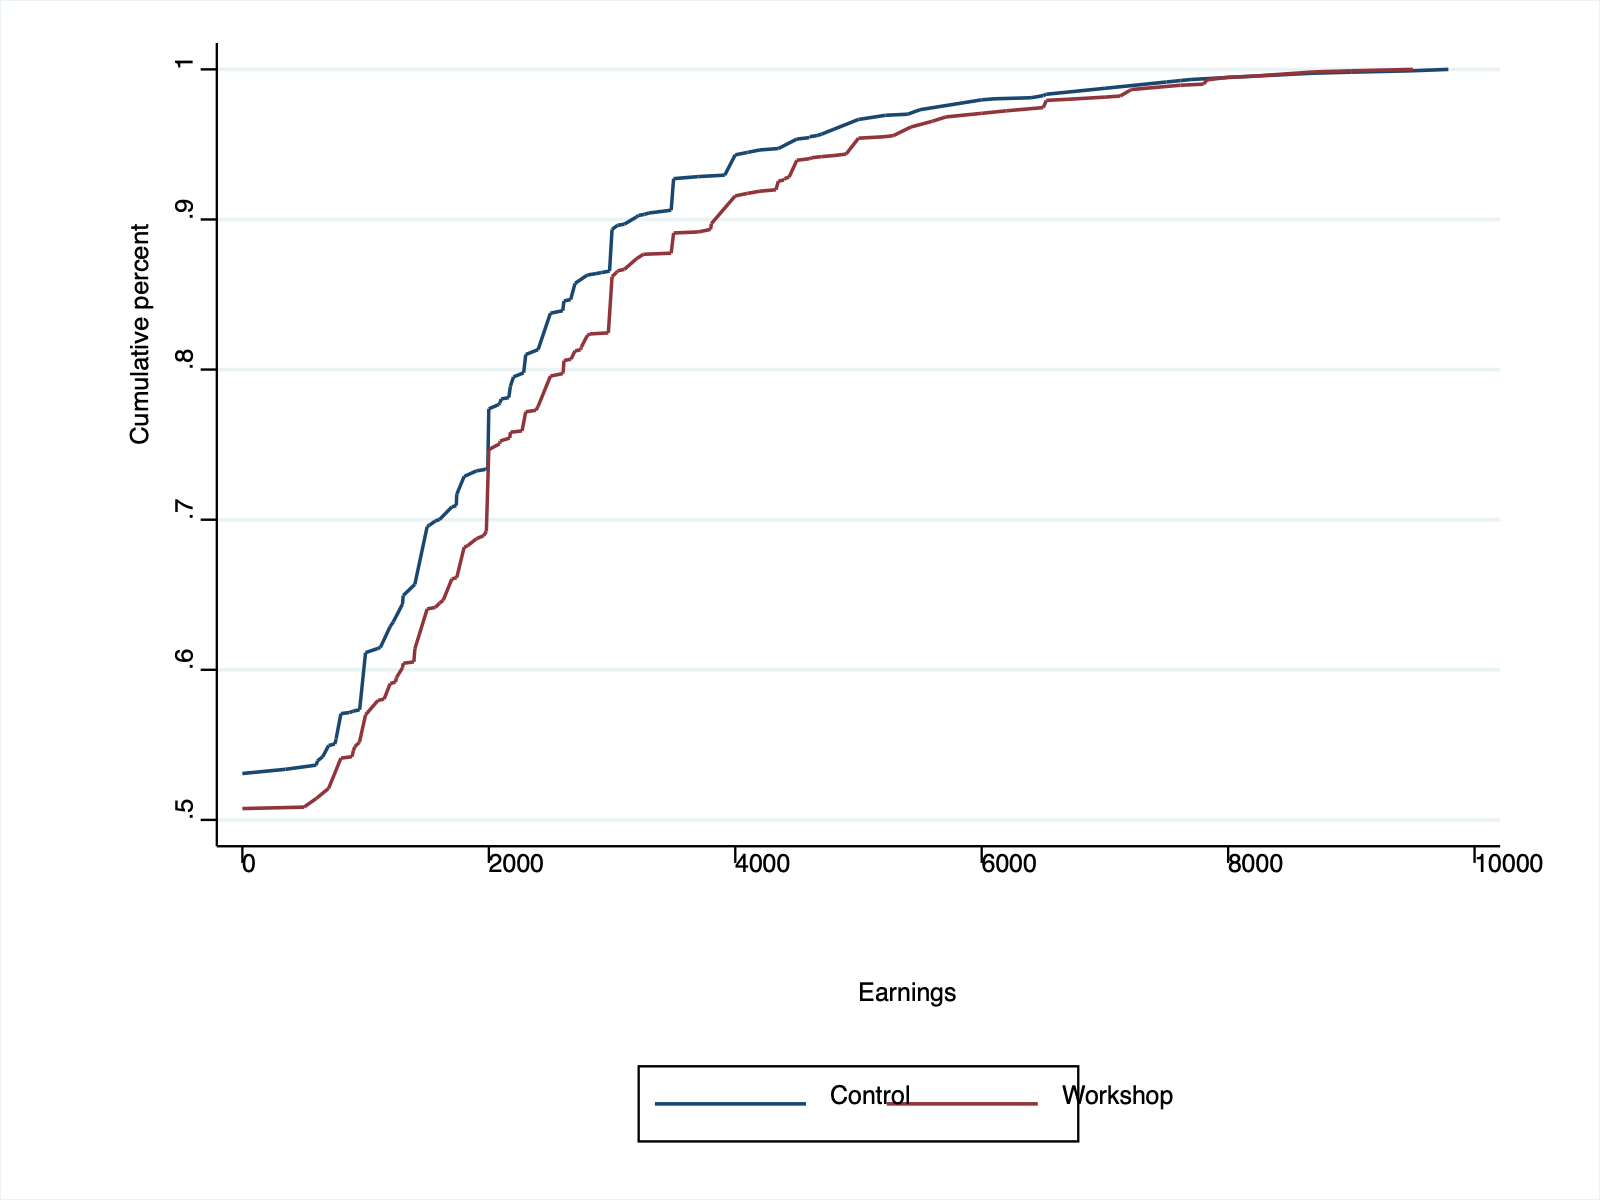
\includegraphics[width=7.5cm,height=5.0cm]{Final Project/Deliverable Final/Figures/Proposed/figure1.png}}
\end{figure}

\noindent First, Figures \ref{fig: figure 1 p} and \ref{fig: figure 1 o} show the distribution of earnings in the second end line for the control and workshop treatment group. This graph shows that earnings for the workshop group are more concentrated to the right across all the distribution. This behaviour shows the importance of quantile regressions on the empirical strategy.  


\begin{figure}[h!]
\censubtering
\caption{Original - Fortnightly impacts of the transport treatment on job search}
  \subfloat[Impact on search \label{fig: figure 1 a orignal}]{\includegraphics[width=7.5cm,height=5.0cm]{Final Project/Deliverable Final/Figures/Original/figure1a.png}}\qquad
  \subfloat[Impacts on searching at job boards \label{fig: figure 1 b orignal}]{\includegraphics[width=7.5cm,height=5.0cm]{Final Project/Deliverable Final/Figures/Original/figure1b.png}}
  \label{fig: 1 original}
\end{figure}

\noindent Second, the transport intervention has a positive treatment effect of job search intensity, while the workshop intervention does not affect job search intensity. This behaviour can be seen comparing figures \ref{fig: 1 original} and \ref{fig: 2 original}. In fact, the graphs show that for in the following days after the start of the transport intervention, labour market outcomes increased by 0.5 percentage points (from a 40\% control mean). However, when looking to the workshop intervention (\ref{fig: 2 original}), after the start of the intervention, the labour market outcomes do not defer from the control group. Furthermore, Figure \ref{fig: 1 original} shows that the effect of the transit intervention does not reflect linear effect over time. Additionally, right when the transport subsidy was made available to participants,  visit to the job vacancies boards increased by 9\% in the treatment group compared to the control.

\begin{figure}[h!]
\censubtering
\caption{Proposed - Fortnightly impacts of the transport treatment on job search}
  \subfloat[Impact on search \label{fig: figure 1 a proposed}]{\includegraphics[width=7.5cm,height=5.0cm]{Final Project/Deliverable Final/Figures/Proposed/figure1a.png}}\qquad
  \subfloat[Impacts on searching at job boards \label{fig: figure 1 b proposed}]{\includegraphics[width=7.5cm,height=5.0cm]{Final Project/Deliverable Final/Figures/Proposed/figure1b.png}}
  \label{fig: 1 proposed}
\end{figure}

\medskip

\noindent For further comparison on figures  of the original and proposed changes see section \ref{apendix figures} of the appendix.
\newpage
\bibliography{Referencia.bib}

\newpage
\appendix
\section{Tables} \label{apendix tables}
%% Table 6 of Abebe et al (2021) ----------------------------------------------

\import{Final Project/Deliverable Final/Tables/Original/}{table6}\label{tab:FD table 6 o}
\import{Final Project/Deliverable Final/Tables/Proposed/}{table6}\label{tab:FD table 6 p}

\section{Figures} \label{apendix figures}

% Figure 2 Original -------------------------------------------------------

\begin{figure}[h!]
\censubtering
\caption{Original - Fortnightly impacts of the workshop treatment on job search}
  \subfloat[Impact on search \label{fig: figure 2 b orignal }]{\includegraphics[width=7.5cm,height=5.0cm]{Final Project/Deliverable Final/Figures/Original/figure2a.png}}\qquad
  \subfloat[Impacts on searching at job boards \label{fig: figure 2 b orignal }]{\includegraphics[width=7.5cm,height=5.0cm]{Final Project/Deliverable Final/Figures/Original/figure2b.png}}
  \label{fig: 2 original}
\end{figure}

% Figure 2 Proposed -------------------------------------------------------

\begin{figure}[h!]
\censubtering
\caption{Proposed - Fortnightly impacts of the workshop treatment on job search}
  \subfloat[Impact on search \label{fig: figure 2 a proposed}]{\includegraphics[width=7.5cm,height=5.0cm]{Final Project/Deliverable Final/Figures/Proposed/figure2a.png}}\qquad
  \subfloat[Impacts on searching at job boards \label{fig: figure 2 b proposed}]{\includegraphics[width=7.5cm,height=5.0cm]{Final Project/Deliverable Final/Figures/Proposed/figure2b.png}}
  \label{fig: 2 proposed}
\end{figure}

% Figure 5A Original -------------------------------------------------------

\begin{figure}[h!]
\censubtering
\caption{Original - Fortnightly impacts of the workshop treatment on job search}
  \subfloat[Impact on search \label{fig: figure 2 b orignal }]{\includegraphics[width=7.5cm,height=5.0cm]{Final Project/Deliverable Final/Figures/Original/figure5a.png}}\qquad
  \subfloat[Impacts on searching at job boards \label{fig: figure 2 b orignal }]{\includegraphics[width=7.5cm,height=5.0cm]{Final Project/Deliverable Final/Figures/Original/figure5b.png}}
  \label{fig: 2 original}
\end{figure}

% Figure 5A Proposed -------------------------------------------------------

\begin{figure}[h!]
\censubtering
\caption{Proposed - Fortnightly impacts of the workshop treatment on job search}
  \subfloat[Impact on search \label{fig: figure 2 a proposed}]{\includegraphics[width=7.5cm,height=5.0cm]{Final Project/Deliverable Final/Figures/Proposed/figure5a.png}}\qquad
  \subfloat[Impacts on searching at job boards \label{fig: figure 2 b proposed}]{\includegraphics[width=7.5cm,height=5.0cm]{Final Project/Deliverable Final/Figures/Proposed/figure5b.png}}
  \label{fig: 2 proposed}
\end{figure}

\end{document}